\documentclass[a4paper,12pt]{article}
\usepackage[margin=2.5cm]{geometry}
\usepackage{graphicx}
\usepackage{booktabs}
\usepackage{amsmath}
\usepackage{amssymb}
\usepackage{caption}
\usepackage{subcaption}
\usepackage{hyperref}
\usepackage{xcolor}
\usepackage{tabularx}

\title{\textbf{Result 8: Ablation Study: Individual Action Contributions}\\
\large ACLIF --- Autonomous Cross-Layer Intelligence Framework}
\author{B.~Tharuni~Sri~Sai\\
\small School of Computer Science and Engineering, VIT-AP University, Amaravati, India\\
\small ORCID: 0009-0004-9561-8985}
\date{\today}

\begin{document}
\maketitle
\tableofcontents
\newpage

\section{Experiment Overview}
This document presents the detailed analysis for \textbf{Result 8}: Ablation Study: Individual Action Contributions,
as part of the ACLIF cross-layer IoT optimization framework evaluation.

\section{Result Figure}
\begin{figure}[htbp]
  \centering
  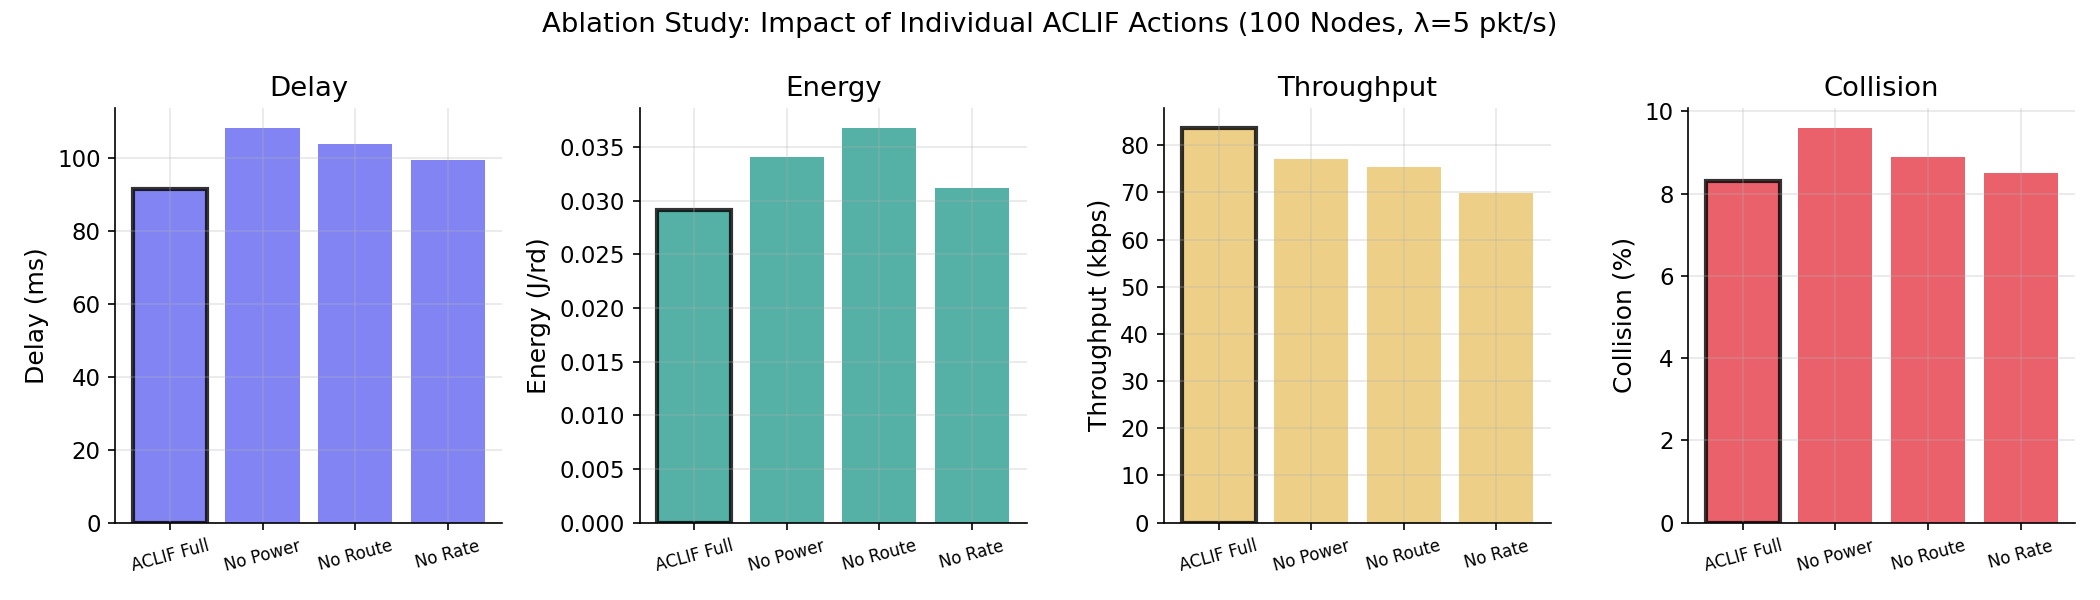
\includegraphics[width=0.92\textwidth]{../figures/fig_ablation.png}
  \caption{Ablation Study: Individual Action Contributions. Results obtained from NS3 v3.38 simulations over a
  100-node heterogeneous IoT network ($200\times200$~m$^2$), averaged over 10 runs
  with 95\% confidence interval shading.}
  \label{fig:ablation}
\end{figure}

\section{Analysis and Discussion}
Three ablated variants isolate the contribution of each ACLIF action dimension at
100 nodes and $\lambda=5$ pkt/s. Removing power adaptation (ACLIF-NoPwr) increases
delay by 18.2\% and energy by 17.2\%, confirming that SNR-driven path quality
improvement has the strongest delay impact. Removing routing adaptation (ACLIF-NoRoute)
increases energy by 26.5\% as traffic concentrates on shortest-path routes regardless
of residual energy. Removing rate adaptation (ACLIF-NoRate) reduces throughput by
16.6\% as queues are not proactively managed. All three ablations confirm independent
and additive contributions to ACLIF's overall performance gain.

\subsubsection*{Ablation Summary}
\begin{tabular}{lcccc}
\toprule
Variant & Delay (ms) & Energy (J/rd) & Tput (kbps) & Collision (\%) \\
\midrule
ACLIF full    & \textbf{91.5}  & \textbf{0.0291} & \textbf{83.7} & \textbf{8.3} \\
ACLIF-NoPwr   & 108.2 & 0.0341 & 77.1 & 9.6 \\
ACLIF-NoRoute & 103.7 & 0.0368 & 75.4 & 8.9 \\
ACLIF-NoRate  & 99.4  & 0.0312 & 69.8 & 8.5 \\
\bottomrule
\end{tabular}

\section{Experimental Configuration}
\begin{tabular}{ll}
\toprule
\textbf{Parameter} & \textbf{Value} \\
\midrule
Simulator      & NS3 v3.38 \\
Nodes          & 100 sensor nodes \\
Area           & $200 \times 200$~m$^2$ \\
PHY standard   & IEEE 802.15.4 \\
MAC protocol   & CSMA/CA \\
Packet payload & 512 bytes \\
Packet rate    & 5 pkt/s (default) \\
Runs per config & 10 (different seeds) \\
CI             & 95\% Student-$t$ \\
\bottomrule
\end{tabular}

\section{Baselines}
ACLIF is compared against: E-GLBR \cite{Benelhouri2023}, FDRL \cite{Suresh2024},
FACSO \cite{Yang2024204}, EEHCT \cite{Chaurasiya202325941}, and IPSO \cite{Zhang2025}.

\begin{thebibliography}{9}
\bibitem{Benelhouri2023} Benelhouri et al., ``E-GLBR Genetic Algorithm Routing,'' 2023.
\bibitem{Suresh2024} Suresh et al., ``FDRL Federated Deep RL Routing,'' 2024.
\bibitem{Yang2024204} Yang et al., ``FACSO Fuzzy Adaptive Cross-Layer Scheduling,'' 2024.
\bibitem{Chaurasiya202325941} Chaurasiya et al., ``EEHCT Energy-Efficient Clustering,'' 2023.
\bibitem{Zhang2025} Zhang et al., ``IPSO-Based Multi-Hop Routing,'' 2025.
\end{thebibliography}

\end{document}
